\documentclass[tikz,border=10pt]{standalone}
\usepackage{amssymb}
\begin{document}
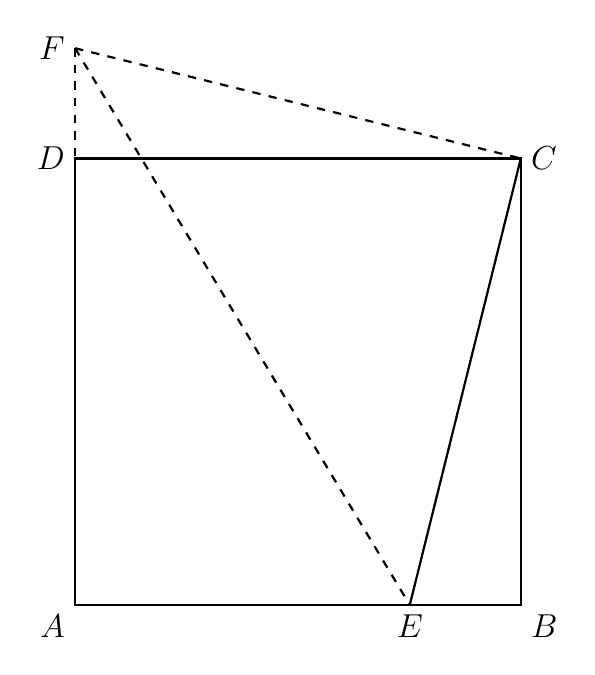
\begin{tikzpicture}[line width=0.8pt, font=\large]
  \coordinate (A) at (0,0);
  \coordinate (B) at (5.66,0);
  \coordinate (C) at (5.66,5.67);
  \coordinate (D) at (0,5.67);
  \coordinate (E) at (4.25,0);
  \coordinate (F) at (0,7.07);

  \draw (A) -- (B) -- (C) -- (D) -- cycle;
  \draw (E) -- (C);
  \draw[dashed] (F) -- (E);
  \draw[dashed] (F) -- (C);
  \draw[dashed] (F) -- (D);

  \node[below left] at (A) {$A$};
  \node[below right] at (B) {$B$};
  \node[right] at (C) {$C$};
  \node[left] at (D) {$D$};
  \node[below] at (E) {$E$};
  \node[left] at (F) {$F$};
\end{tikzpicture}
\end{document}
